\documentclass[8pt]{beamer}
\mode<presentation> {
    \usetheme{Copenhagen}
}

\usepackage{graphicx}
\usepackage{booktabs} 
\usepackage{graphicx,wrapfig,lipsum}
\usepackage{ragged2e}
\usepackage{etoolbox}
\usepackage[absolute,overlay]{textpos}

\title[Adversarial Machine Learning]{Adversarial Machine Learning:\\ problem evaluation and implementation} 

\medskip
\institute[UniBG] 
{\Large
    University of Bergamo \\Department of Engineering \\ 
    \vspace{0.5cm}
    \medskip
    \textit{Computer Security \\AY 20/21}
}

\vspace{0.5cm}
\author{Luca Ghislotti}
\date{\today}

\begin{document}

\begin{frame}
\titlepage
\end{frame}

\begin{frame}
\frametitle{Overview}
\tableofcontents
\end{frame}

\section{The problem} 
\subsection{A spot of context}
\begin{frame}{A spot of context}
\begin{columns}
\begin{column}{0.55\textwidth}
    \begin{center}
        \begin{figure} 
        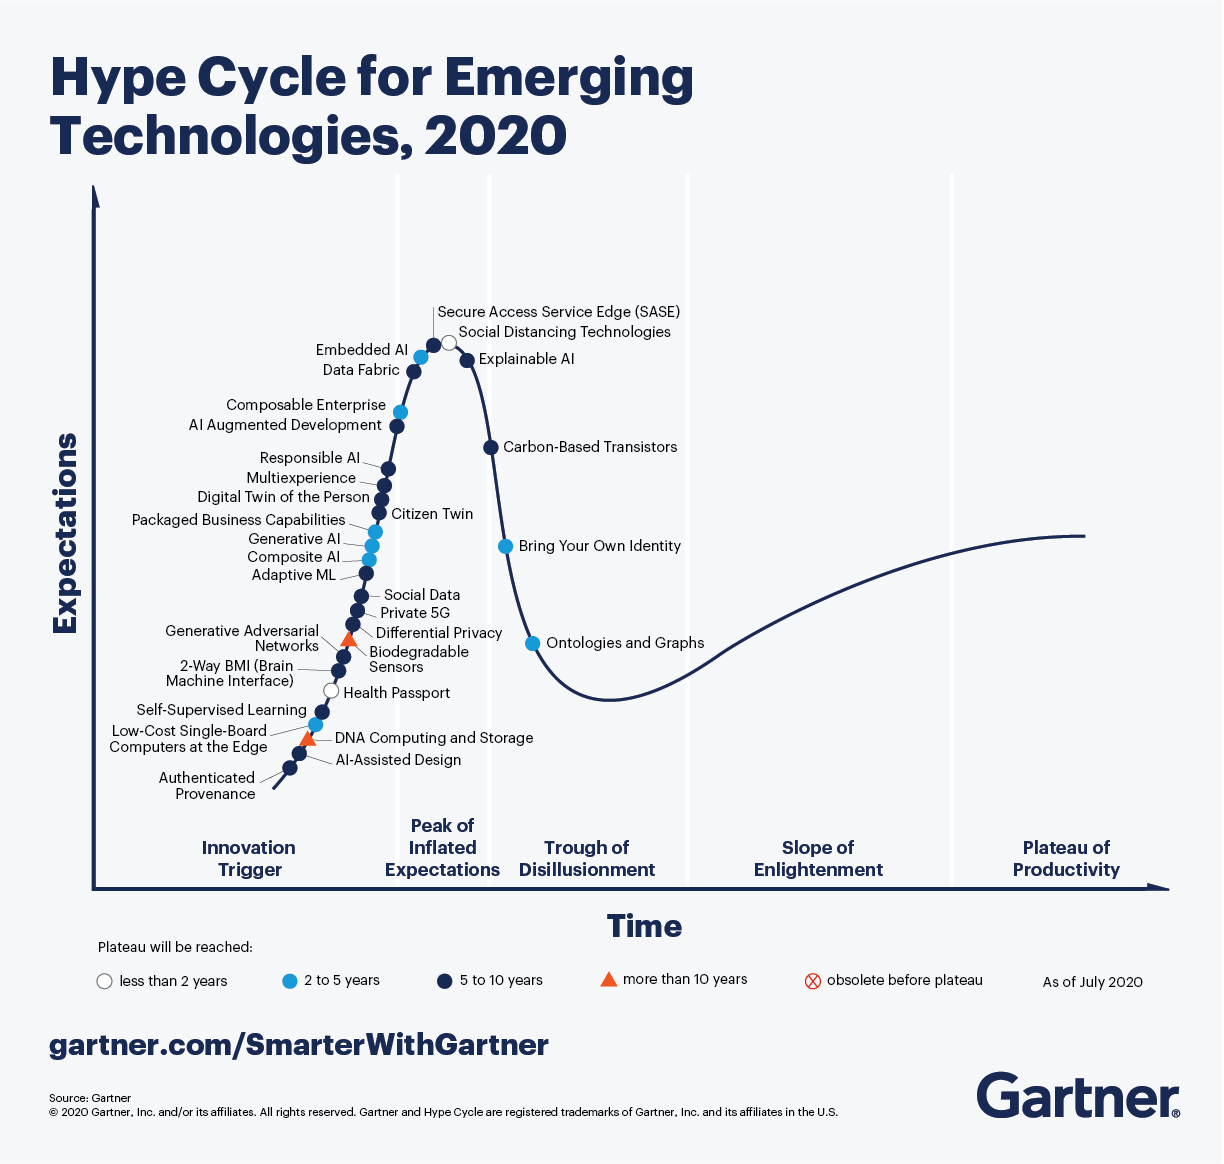
\includegraphics[scale=0.12]{images/hypegraph.png}
        \caption{Gartner hype cycle for emerging technologies}
        \end{figure}
    \end{center}
\end{column}

\begin{column}{0.45\textwidth}
As machine learning techniques have entered computing mainstream, their uses have multiplied. Online advertising and algorithmic trading are now inconceivable without machine learning, and machine learning techniques are increasingly finding their ways into health informatics, fraud detection, computer vision, machine translation, and natural language understanding.
\vspace{0.5cm}
\end{column}
\end{columns}
\end{frame}

\subsection{What do we mean with Adversarial Machine Learning?}
\begin{frame}
\frametitle{What do we mean with Adversarial Machine Learning?}
\begin{figure} 
    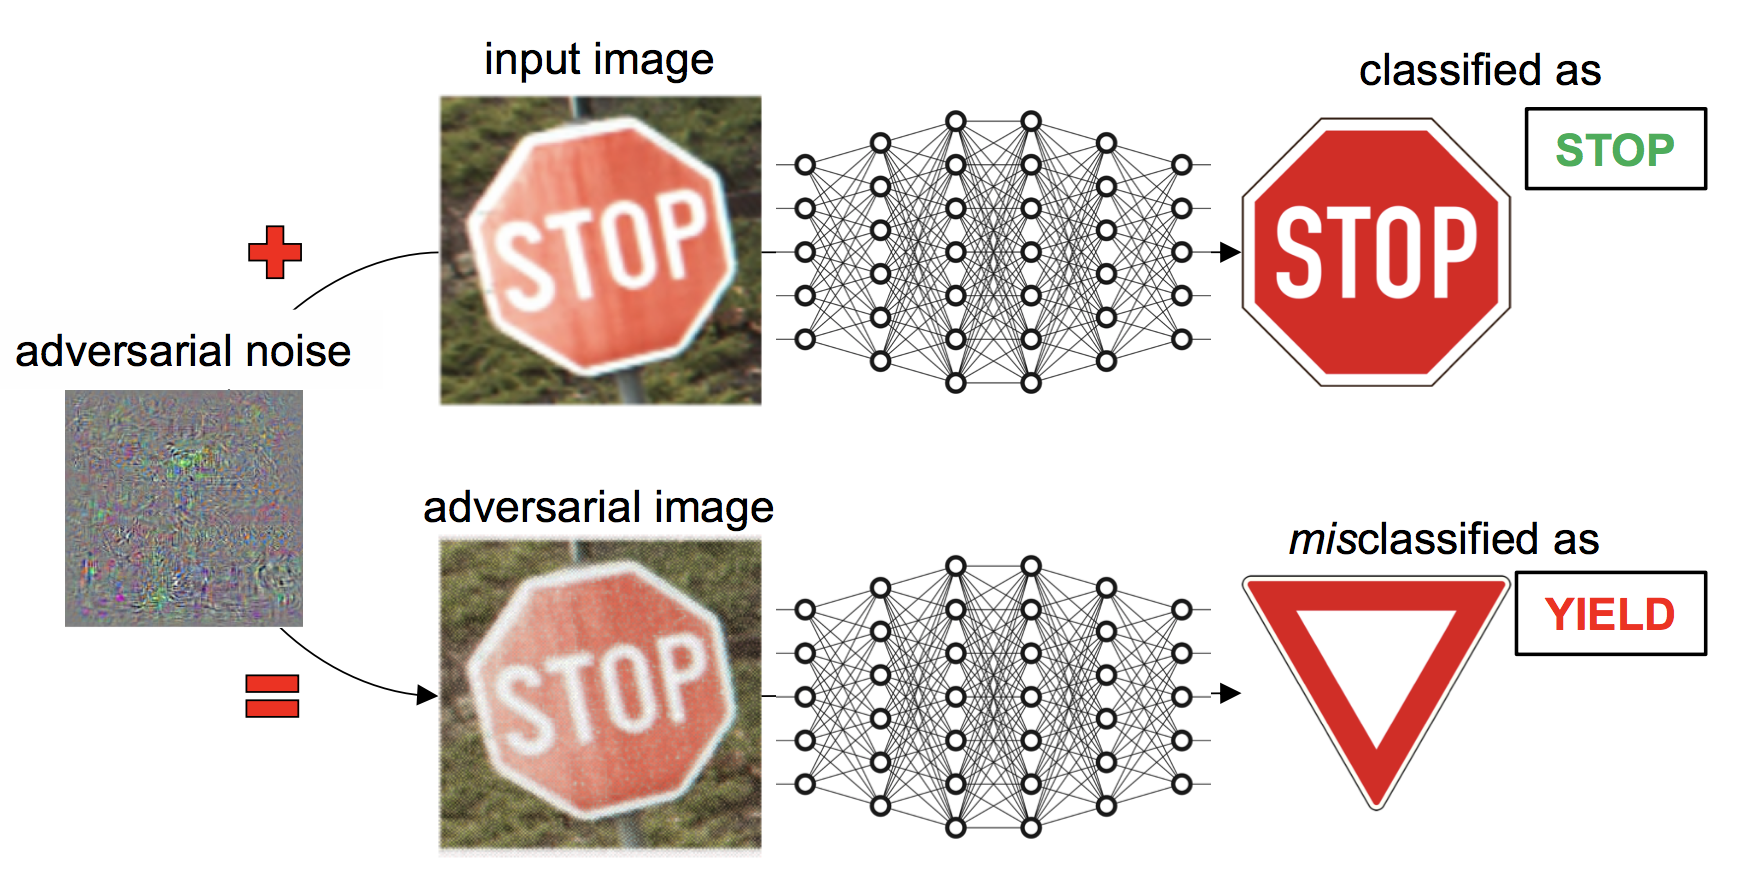
\includegraphics[scale=0.25]{images/adv_stop.png}
    \caption{An example of image manipulation}
\end{figure}
Many applications of machine learning are adversarial in nature. Some are adversarial because they are safety critical, such as autonomous driving. An adversary in these applications can be a malicious party aimed at causing congestion or accidents, or may even model unusual situations that expose vulnerabilities in the prediction engine.
\end{frame}

\subsection{Why is it such an important issue?}
\begin{frame}
\frametitle{Why is it such an important issue?}
\begin{columns}
    \begin{column}{0.6\textwidth}
        One potential concern with learning algorithms is that they may introduce a security fault into systems that employ them. The key strengths of learning approaches are their adaptability and ability to infer patterns that can be used for predictions and decision making. However, these advantages of machine learning can potentially be subverted by adversarial manipulation of the knowledge and evidence provided to the learner.
        \\~\\
        In rapidly changing environments, machine learning techniques are considerably advantageous over handcrafted rules and other approaches because they can infer hidden patterns in data, they can adapt quickly to new signals and behaviors, and they can provide statistical soundness to a decision-making process.
    \end{column}
    \begin{column}{0.4\textwidth}
    \begin{center}
        \begin{figure} 
        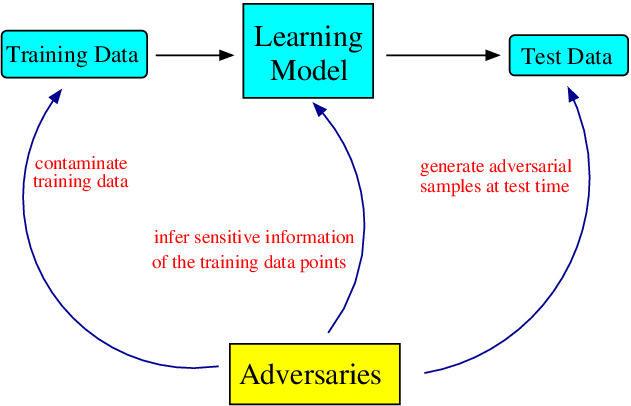
\includegraphics[scale=0.25]{images/adv_cycle.jpg}
        \caption{Different points of interaction between the adversary and the system}
        \end{figure}
    \end{center}
\end{column}
\end{columns}

\end{frame}

\subsection{Different ways to implement an attack}
\begin{frame}
\frametitle{Different ways to implement an attack}
We classify attacks along three dimensions: \textit{timing}, \textit{information}, and \textit{goals}.
\begin{block}{The \textit{timing} dimension}
    The first crucial consideration in modeling attacks is \textit{when} the attack takes place. \textbf{Attacks on models} assume that the model has already been learned, and the attacker now either changes its behavior, or makes changes to the observed environment, to cause the model to make erroneous predictions. \textbf{Poisoning attacks}, in contrast, take place before models are trained, modifying a part of the data used for training.
\end{block}
\end{frame}

\begin{frame}{Different ways to implement an attack}
    \begin{figure} 
    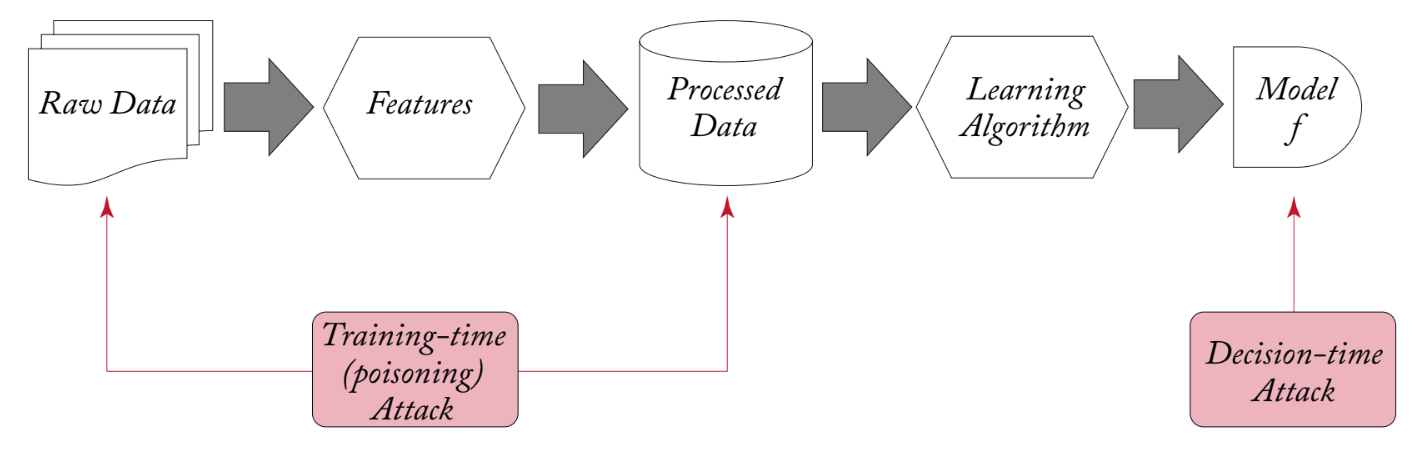
\includegraphics[scale=0.2]{images/attack_dim.png}
    \caption{A schematic representation of the distinction between decision-time attacks (attacks on models) and poisoning attacks (attacks on algorithms)}
\end{figure}
\end{frame}

\begin{frame}{Different ways to implement an attack}
\begin{block}{The \textit{information} dimension}
The second important issue in modeling attacks is what information the attacker has about the learning model or algorithm, a distinction which is commonly distilled into white-box vs black-box attacks. In particular, \textbf{white-box attacks} assume that either the model (in the case of attacks on decisions) or algorithm (in poisoning attacks) is fully known to the adversary, whereas in \textbf{black-box attacks} the adversary has limited or even no information at all.
\end{block}
\end{frame}

\begin{frame}{Different ways to implement an attack}
\begin{block}{The \textit{goals} dimension}
Attackers may have different reasons for attacking, such as evading detection or
reducing confidence in the algorithm. We differentiate two broad classes of attack goals: targeted attacks and reliability attacks. In a \textbf{targeted attack}, the attacker’s goal is to cause a mistake on specific instances of a specific nature. A \textbf{reliability attack}, in contrast, aims to degrade the perceived reliability of the learning system by maximizing prediction error.
\end{block}
\end{frame}


\section{Implementation: an example}
\subsection{Project setup: the tools you'll need}
\begin{frame}{}
\Huge{\centerline{Implementation: an example}}
\end{frame}
\begin{frame}
\frametitle{Project setup: the tools you'll need}
In order to try out and test the project you'll need:
\vspace{0.3cm}
\begin{itemize}
    \setlength\itemsep{1em}
    
    \item \textbf{Python 3}
    
    \item \textbf{Tensorflow (2.2 required, 2.4.1 provided)} Free and open-source software library for machine learning. \href{https://www.tensorflow.org/}{\textit{https://tensorflow.org/}}
    
    \item \textbf{Keras (2.2 required, 2.4.3 provided)} Open-source software library that provides a Python interface for artificial neural networks. \href{https://keras.io/}{\textit{https://keras.io/}}
    
    \item \textbf{Matplotlib (3.3 required, 3.3.4 provided)} Comprehensive library for creating static, animated, and interactive visualizations in Python. \href{https://matplotlib.org/}{\textit{https://matplotlib.org/}}
    
    \item \textbf{Conda/Conda-Navigator GUI (optional)} Package, dependency and environment manager. \href{https://docs.conda.io/projects/conda/en/latest/index.html}{\textit{https://docs.conda.io/projects/conda/en/latest/index.html}}
\end{itemize}
\vspace{0.5cm}
Everything's available for Windows/MacOS/Linux (Pop!\_OS 20.10 Kernel 5.8 used)
\end{frame}


\subsection{An example: a Ferrari that turns out to be a purse}
\begin{frame}
\frametitle{An example: a Ferrari that turns out to be a purse}
This example wants to be a very simple implementation of a type of attack, called \textit{Fast Gradient Sign Method} or \textit{FGSM}. The fast gradient sign method works by using the gradients of the neural network to create an adversarial example.
\\~\\
For an input image, the method uses the gradients of the loss with respect to the input image to create a new image that maximises the loss. This new image is called the adversarial image.
\\~\\
This can be summarised using the following expression:\\
\vspace{0.1cm}
\begin{center}
$
adv_x=x+\epsilon \cdot sign(\nabla_x \cdot J(\theta, x, y))
$
\end{center}
Where:\\
\quad - $adv_x$: adversarial image\\
\quad - $J$: loss\\
\quad - $x$: original input image\\
\quad - $y$: original input label\\
\quad - $\epsilon$: multiplier to ensure the perturbations are small\\
\quad - $\theta$: model parameters
\end{frame}


\begin{frame}{An example: a Ferrari that turns out to be a purse}
\begin{figure} 
    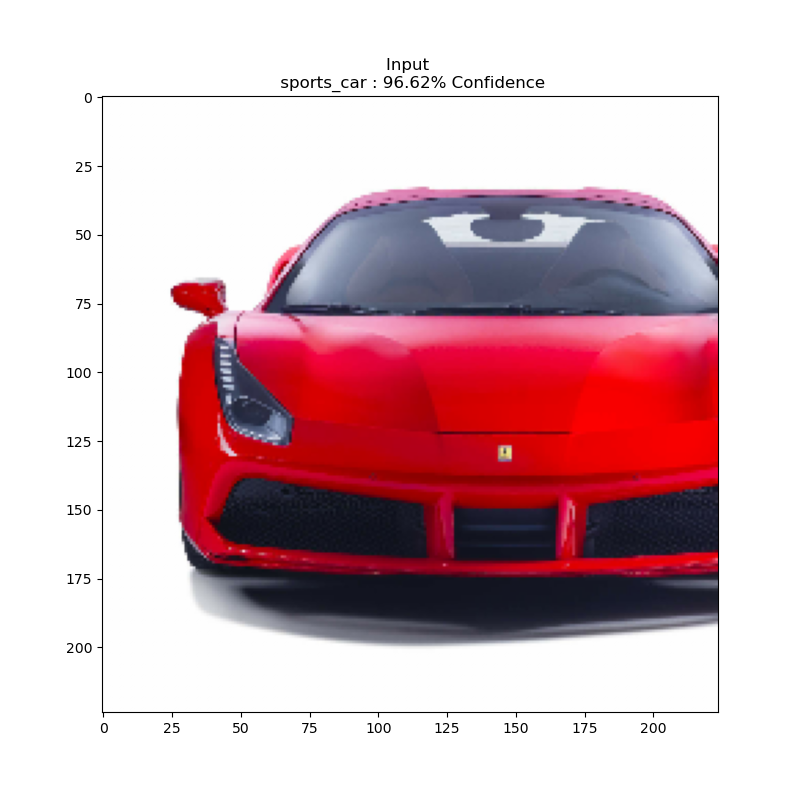
\includegraphics[scale=0.3]{images/input.png}
    \vspace*{-5mm}
    \caption{Input image}
\end{figure}
\end{frame}

\begin{frame}{An example: a Ferrari that turns out to be a purse}
\begin{figure} 
    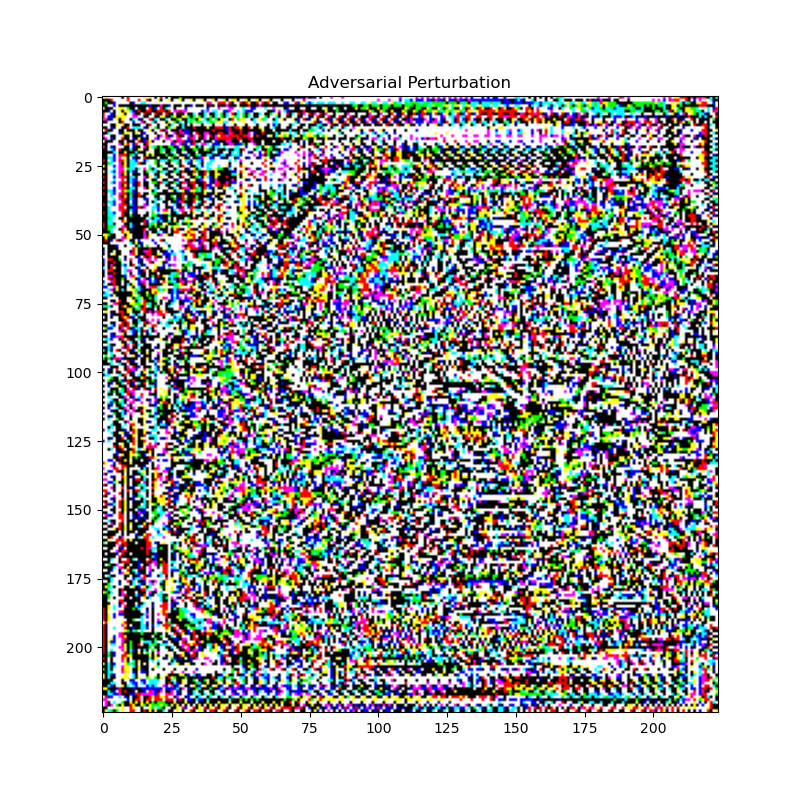
\includegraphics[scale=0.3]{images/perturbation.png}
    \vspace*{-5mm}
    \caption{Perturbation matrix}
\end{figure}
\end{frame}

\begin{frame}{An example: a Ferrari that turns out to be a purse}
\begin{figure} 
    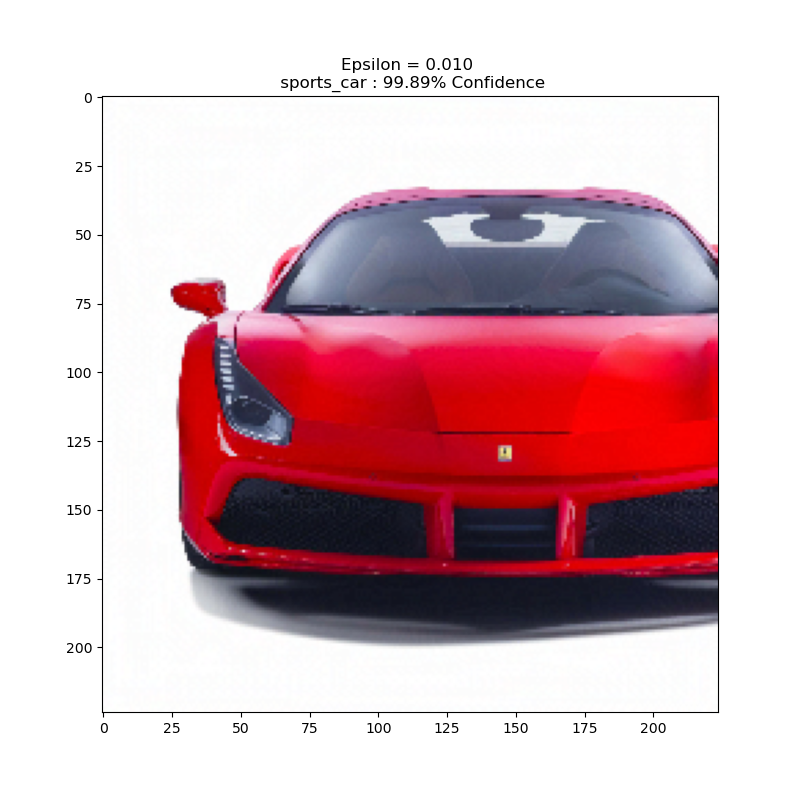
\includegraphics[scale=0.3]{images/output_1.png}
    \vspace*{-5mm}
    \caption{Output image after perturbation with $\epsilon=0.010$}
\end{figure}
\end{frame}

\begin{frame}{An example: a Ferrari that turns out to be a purse}
\begin{figure} 
    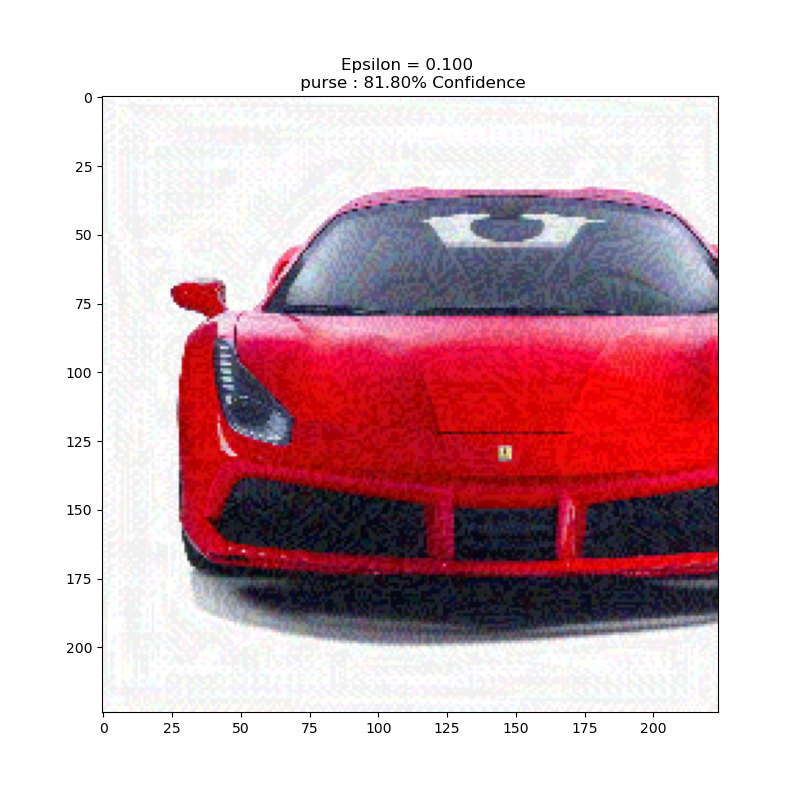
\includegraphics[scale=0.3]{images/output_2.png}
    \vspace*{-5mm}
    \caption{Output image after perturbation with $\epsilon=0.100$}
\end{figure}
\end{frame}

\begin{frame}{An example: a Ferrari that turns out to be a purse}
\begin{figure} 
    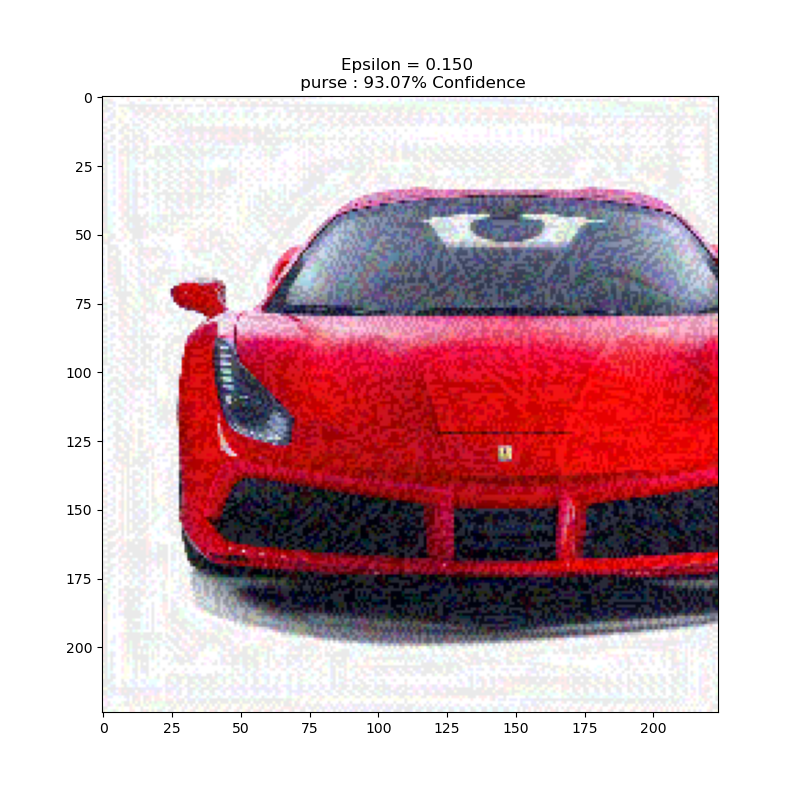
\includegraphics[scale=0.3]{images/output_3.png}
    \vspace*{-5mm}
    \caption{Output image after perturbation with $\epsilon=0.150$}
\end{figure}
\end{frame}


\section{References}
\begin{frame}
\frametitle{References}
\begin{thebibliography}{99}
\bibitem{}{Laskov, Pavel and Richard Lippmann}
\newblock Machine Learning in Adversarial Environments
\newblock \emph{Machine Learning, vol. 81, no. 2, Nov. 2010, pp. 115–19}
\end{thebibliography}

\begin{thebibliography}{99}
\bibitem{}{McDaniel, Patrick, et al.}
\newblock Machine Learning in Adversarial Settings
\newblock \emph{EEE Security \& Privacy, vol. 14, no. 3, May 2016}
\end{thebibliography}

\begin{thebibliography}{99}
\bibitem{}{Tygar, J. D}
\newblock Adversarial Machine Learning
\newblock \emph{IEEE Internet Computing, vol. 15, no. 5, Sept. 2011, pp. 4–6}
\end{thebibliography}

\end{frame}

\begin{frame}{A book suggestion}
    \begin{figure} 
    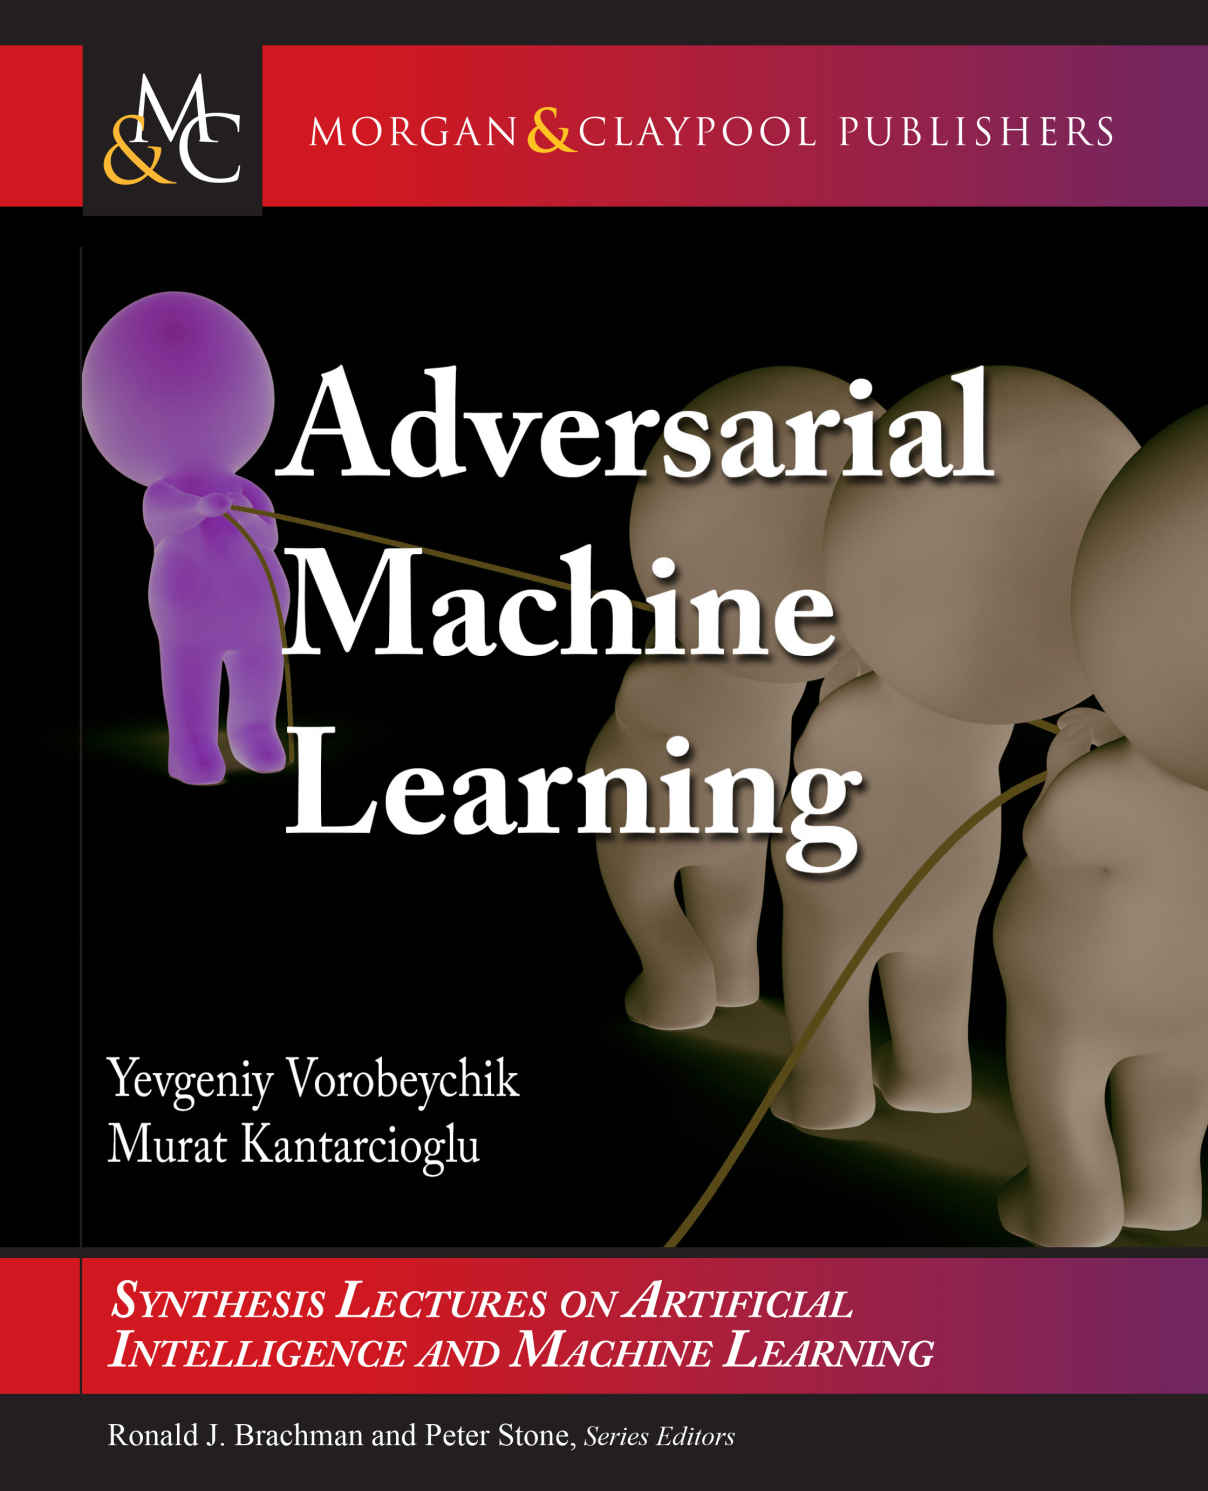
\includegraphics[scale=0.4]{images/adv_book.jpg}
    \caption{Adversarial Machine Learning: Synthesis Lectures on Artificial Intelligence and Machine Learning. Yevgeniy Vorobeychik and Murat Kantarcioglu. Morgan \& Claypool, 2018}
    \end{figure}
\end{frame}

\begin{frame}
\frametitle{Useful links}
\begin{itemize}
\item \textbf{GitHub Project}\\\href{https://github.com/lucaghislo/adversarial_machine_learning}{\textit{https://github.com/lucaghislo/adversarial\_machine\_learning}}
\vspace{0.5cm}
\item \textbf{LaTeX Project}\\\href{https://it.overleaf.com/read/kfkrrytsqpzw}{\textit{https://it.overleaf.com/read/kfkrrytsqpzw}}
\end{itemize}
\end{frame}

\begin{frame}
\Huge{\centerline{The End}}
\end{frame}

\end{document} 